\section{Thực nghiệm}
\subsection{Miêu tả bộ dữ liệu}
\subsection{Phương pháp tổ chức dữ liệu thực nghiệm}
\subsubsection{Dịch bảng}
Trong quá trình chuyển ngữ từ Trung sang Việt, chúng em đã tận dụng thư viện "googletrans" - một công cụ Python không mất phí và không giới hạn số lần dịch. Thư viện này vận hành thông qua API Google Translate Ajax để thực hiện các tác vụ như nhận diện ngôn ngữ và dịch thuật.\\
\\
Do khối lượng dữ liệu lớn, quá trình dịch gặp phải một số thách thức về thời gian và kết nối. Để khắc phục, chúng em đã triển khai các giải pháp sau:
\begin{quote}
\begin{itemize}
    \item Lưu lại tiến trình dịch để tránh mất dữ liệu
    \item Thiết lập cơ chế tự động gửi lại yêu cầu khi mất kết nối
    \item Ứng dụng thư viện "asyncio" cho phép gửi đồng thời nhiều API, giúp tối ưu tốc độ xử lý
\end{itemize}
\end{quote}
Đây là một phần code mẫu đã sử dụng phương pháp đã nêu trên:\\
\begin{figure}[h]
    \centering
    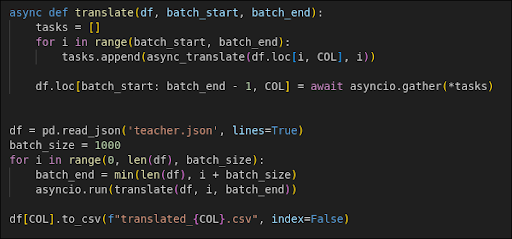
\includegraphics[width=0.75\linewidth]{figures/1.png}
\end{figure}
\newpage
Ngoài ra, chúng em nhận thấy không cần thiết phải dịch toàn bộ các trường dữ liệu lớn để huấn luyện mô hình vì một số trường dữ liệu không hỗ trợ cho việc huấn luyện mô hình. Thay vào đó, chúng em chỉ tập trung dịch 1 số trường sau đây:
\begin{quote}
-\textbf{course.json:} dịch cột “name”, “field”, “prerequisites” và “about”\\
\begin{figure}[h]
    \centering
    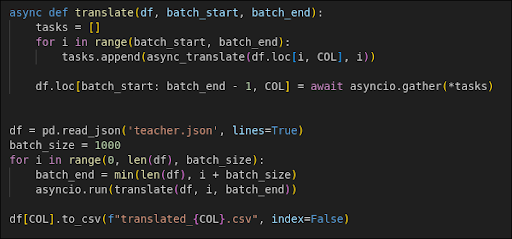
\includegraphics[width=1\linewidth]{figures/2.png}
\end{figure}\\
\\
\\
-\textbf{user.json:} dịch cột “school”\\
\begin{figure}[h]
    \centering
    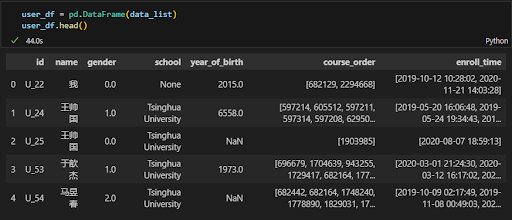
\includegraphics[width=0.8\linewidth]{figures/3.png}
\end{figure}
\newpage
-\textbf{teacher.json:} Tiến hành dịch tất cả (trừ “id” và “name”)\\
\begin{figure}[h]
    \centering
    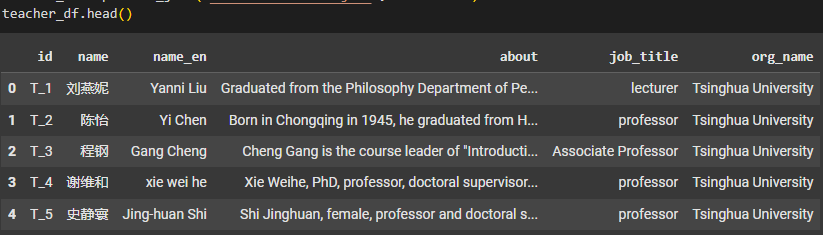
\includegraphics[width=1\linewidth]{figures/4.png}
\end{figure}\\
-\textbf{concept.json:} Dịch tất cả các cột của bảng này vì toàn bộ đều ở dạng chuỗi\\
\begin{figure}[h]
    \centering
    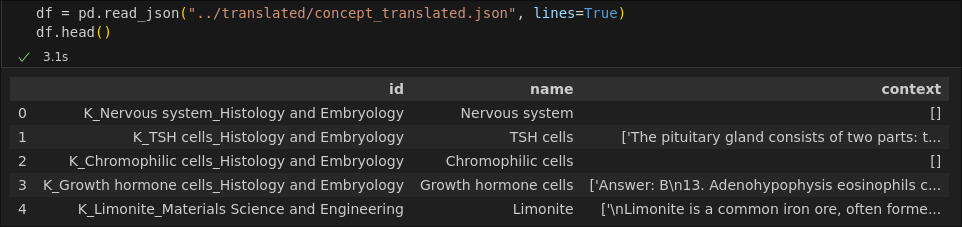
\includegraphics[width=1\linewidth]{figures/5.png}
\end{figure}\\
-\textbf{course-field.json:} Tiến hành dịch cột course\_name và field mang các thông tin dưới dạng chuỗi của bảng.\\
\begin{figure}[h]
    \centering
    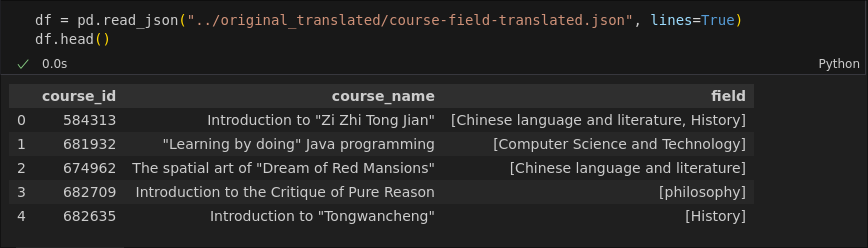
\includegraphics[width=1\linewidth]{figures/6.png}
\end{figure}
\end{quote}
\subsubsection{Khám phá dữ liệu}
\textbf{a) Bảng course.json}\\
Ta xem qua bảng course.json:
\begin{figure}[h]
    \centering
    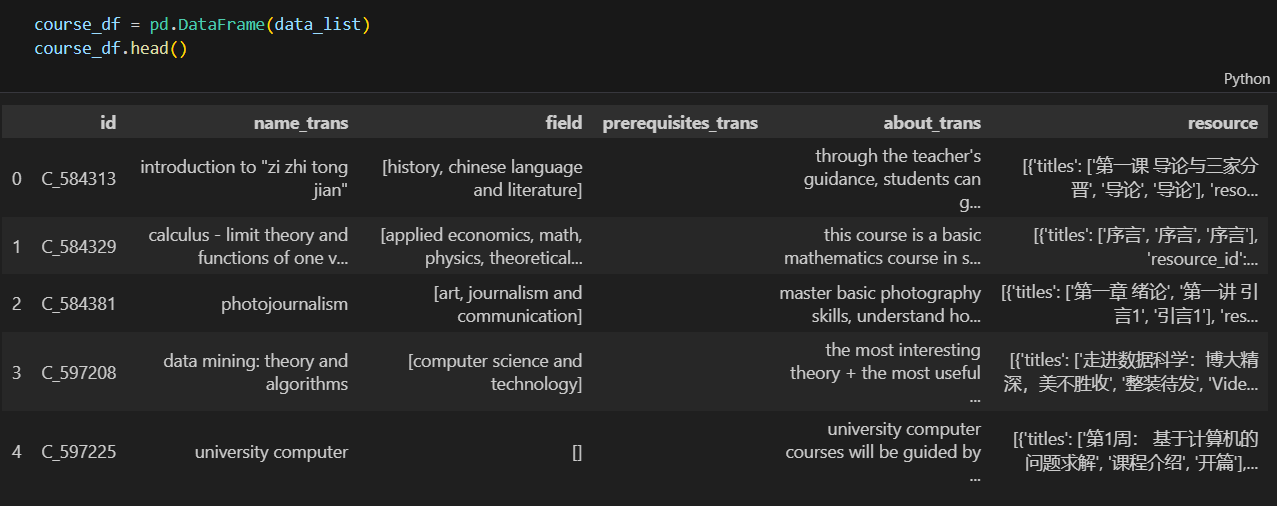
\includegraphics[width=1\linewidth]{figures/7.png}
\end{figure}\\
Ta xét độ dài của 3 cột “about”, “name\_trans” và “resource”:
\begin{figure}[h]
    \centering
    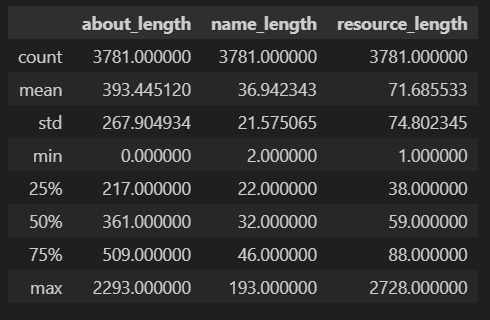
\includegraphics[width=0.485\linewidth]{figures/8.png}
\end{figure}
\newpage
Ta có thể thấy được 1 số thông tin từ dữ liệu trên:
\begin{itemize}
    \item Có những dòng dữ liệu không tồn tại cột “about”, tồn tại giá trị ngoại tệ ở cột “about” vì mean là 393 mà max lên đến 2293. Ta thể hiện trên boxplot độ dài của cột “about”:
    \begin{figure}[h]
        \centering
        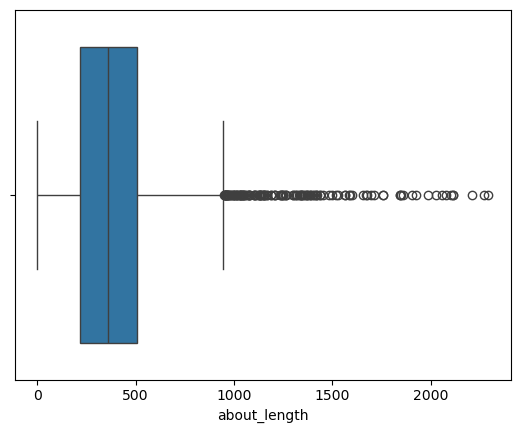
\includegraphics[width=0.75\linewidth]{figures/9.png}
    \end{figure}
    \item Có thể thấy thật sự nhiều giá trị ngoại tệ cần được xử lí.
    \item Có những dòng dữ liệu không có resource\_length, mean cũng rất ngắn (71) chứng tỏ ít thông tin về khoá học.
\end{itemize}
Ta phân tích sâu cột “resource”:
\begin{figure}[h]
    \centering
    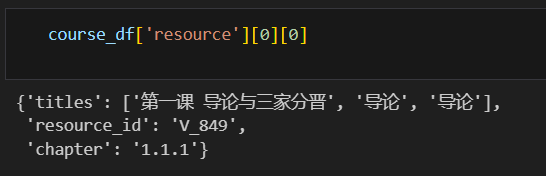
\includegraphics[width=0.75\linewidth]{figures/10.png}
\end{figure}\\
Mỗi resource trong bảng 2 là 1 tập hợp các video hay một tập các exercise. Mỗi resource sẽ có thêm 1 resource\_id là id của resource, chapter là chương chứa resource trong khóa học, titles gồm các tiêu đề như tiêu đề chương, video chương.\\
\\
Thông tin của resource có thể tìm thấy trong file course.json. Một resource có 2 loại: Video và Exercise. Nếu loại tài nguyên là video, nó được xác định bằng ID video bắt đầu bằng ký tự V\_. Nhiều video\_id khác nhau tương ứng với một ccid, và ccid xác định duy nhất một video. Các video\_id này tương ứng với việc hiển thị cùng một video ccid tại các thời gian bắt đầu khác nhau. Mối liên hệ giữa video\_id và ccid được lưu trong relations/video\_id-ccid.txt. Phụ đề video có thể được tìm thấy trong tệp entities/video.json thông qua ccid.\\
\\
Ta sẽ kiểm tra xem có bao nhiêu ID video không hợp lệ để phục vụ cho quá trình xử lý dữ liệu sau này:
\begin{figure}[h]
    \centering
    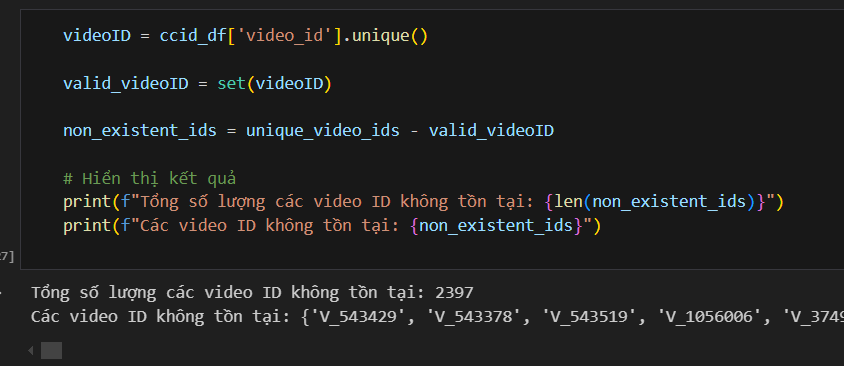
\includegraphics[width=0.75\linewidth]{figures/11.png}
\end{figure}\\
Có 2397 video ID không tồn tại, ta sẽ lọc đi hỗ trợ cho hiển thi thông tin trong tương lai.\\
\\
Ta bắt đầu tiến hành đếm số khoá học trong cột “name\_trans”, chia bởi lĩnh vực (cột “field”):\\
\begin{figure}[h]
    \centering
    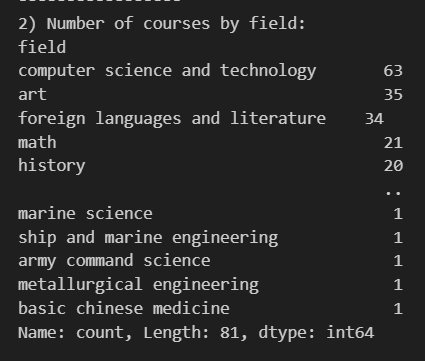
\includegraphics[width=0.35\linewidth]{figures/12.png}
\end{figure}
\newpage
\begin{figure}
    \centering
    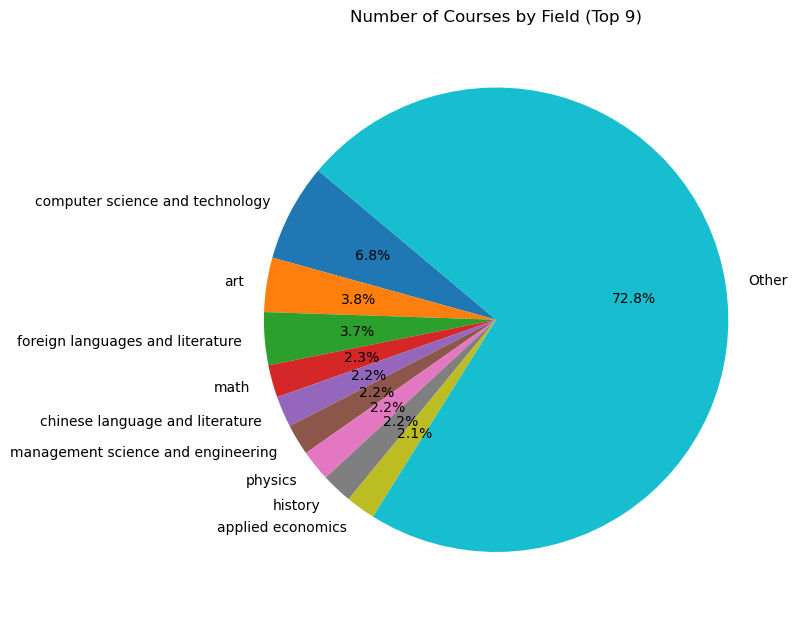
\includegraphics[width=0.7\linewidth]{figures/13.png}
\end{figure}
Ta thấy có tổng 3781 khoá học và 81 lĩnh vực, với “computer science and technology” đứng đầu với 63 khoá học, chiếm 6.8\% trên tổng khoá học. Ta cũng kiểm tra với mỗi khoá học được xếp bao nhiêu lĩnh vực (cột “field”):
\begin{figure}[h]
    \centering
    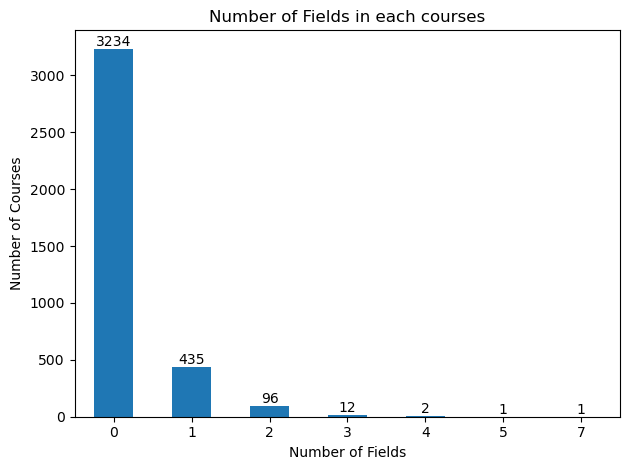
\includegraphics[width=0.9\linewidth]{figures/14.png}
\end{figure}\\
\newpage
Ta có thể thấy có rất nhiều khoá học không thuộc lĩnh vực nào, có rất nhiều khóa học không có field nào, có thể cột “field” sẽ không đóng góp nhiều trong xây dựng thuật toán hoặc cần xử lí.\\
\textbf{b) Bảng user.json}\\
Đầu tiên, ta đọc dữ liệu và quan sát dữ liệu thông qua dạng bảng (DataFrame):
\begin{figure}[h]
    \centering
    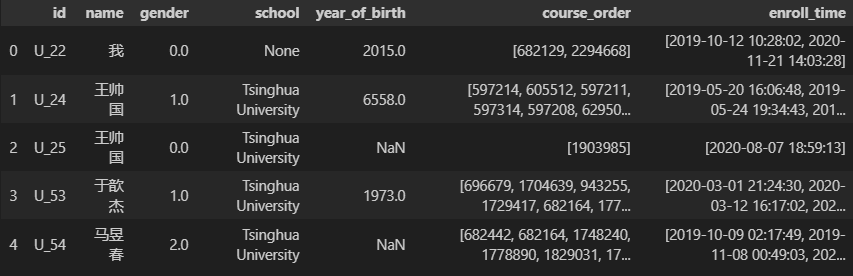
\includegraphics[width=1\linewidth]{figures/15.png}
\end{figure}
\newpage
Ta tiến hành thống kê đặc điểm từng cột có trong bảng:
\begin{figure}[h]
    \centering
    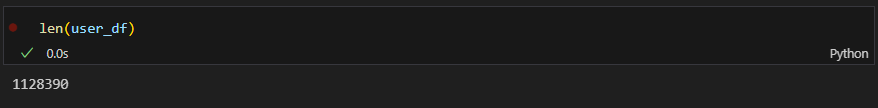
\includegraphics[width=1\linewidth]{figures/16.png}
    \caption{Số lượng users}
\end{figure}
\begin{figure}[h]
    \centering
    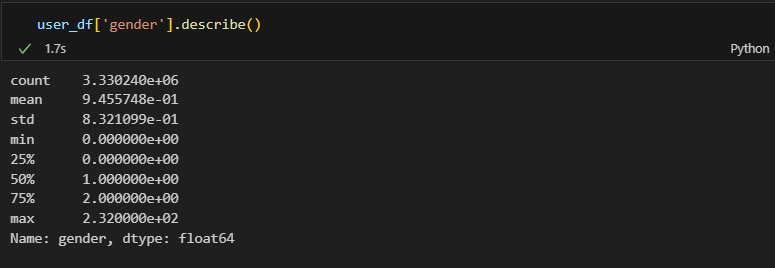
\includegraphics[width=1\linewidth]{figures/17.png}
    \caption{Cột “gender”}
\end{figure}
\begin{figure}[h]
    \centering
    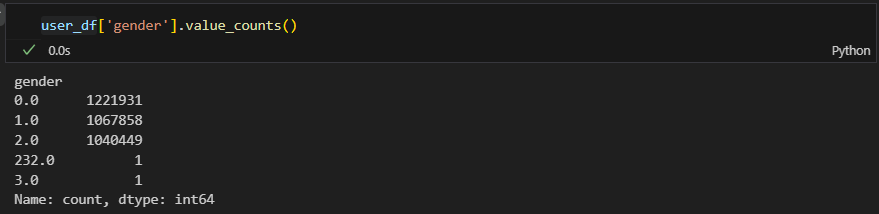
\includegraphics[width=1\linewidth]{figures/18.png}
    \caption{Phân bố các các giá trị trong cột “gender”:}
\end{figure}
\newpage
\begin{figure}
    \centering
    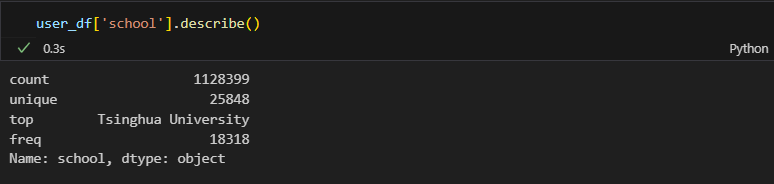
\includegraphics[width=1\linewidth]{figures/19.png}
    \caption{Thông tin cột “school”}
\end{figure}
\begin{figure}[h]
    \centering
    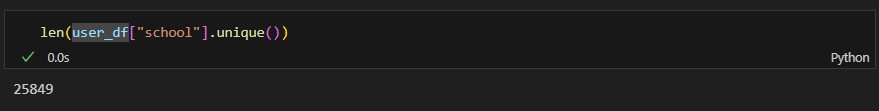
\includegraphics[width=1\linewidth]{figures/20.png}
    \caption{Số lượng trường học trong bảng}
\end{figure}
\begin{figure}[h]
    \centering
    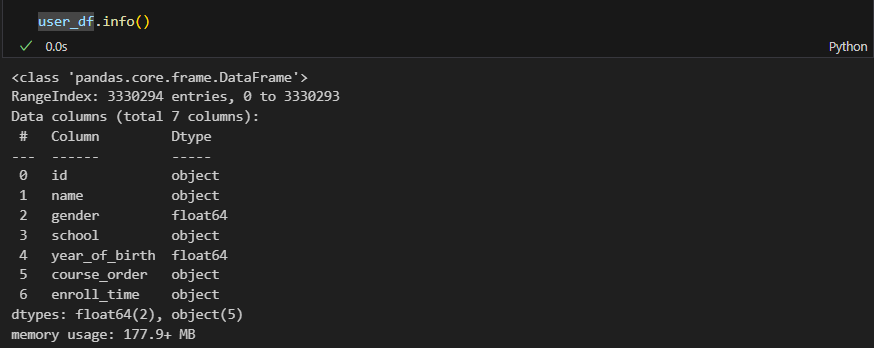
\includegraphics[width=1\linewidth]{figures/21.png}
    \caption{Kiểm tra thông tin tổng quan sau cùng}
\end{figure}
\newpage
\begin{figure}
    \centering
    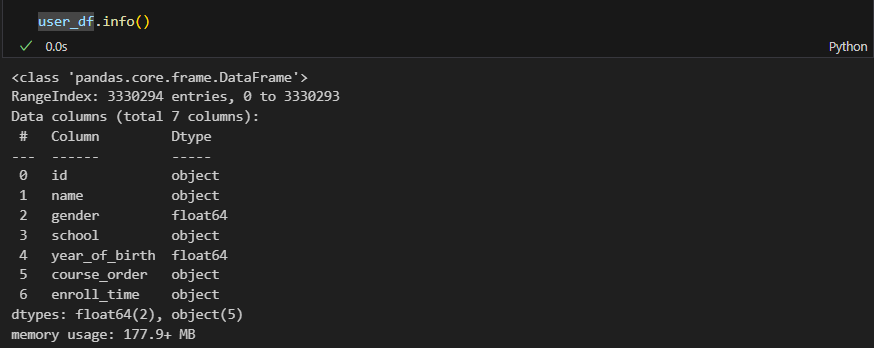
\includegraphics[width=1\linewidth]{figures/22.png}
    \caption{Số lượng sample (users) có trong bảng và số lượng users thuộc về mỗi trường học}
\end{figure}
\begin{figure}[h]
    \centering
    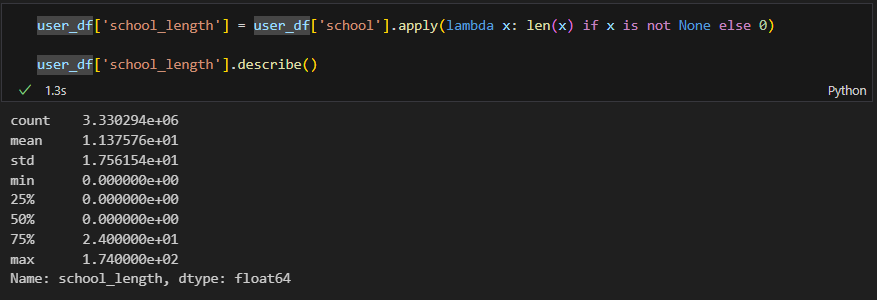
\includegraphics[width=1\linewidth]{figures/23.png}
    \caption{Tạo một cột “school\_length” để phân tích độ dài mỗi sample của cột}
\end{figure}
\newpage
\begin{figure}
    \centering
    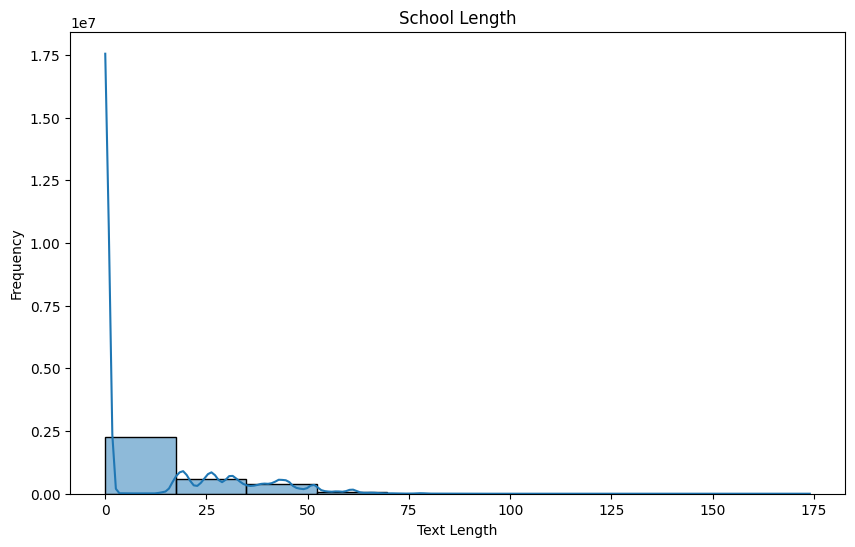
\includegraphics[width=0.68\linewidth]{figures/24.png}
    \caption{Trực quan hóa độ dài của sample cột “school”}
\end{figure}
\begin{figure}[h]
    \centering
    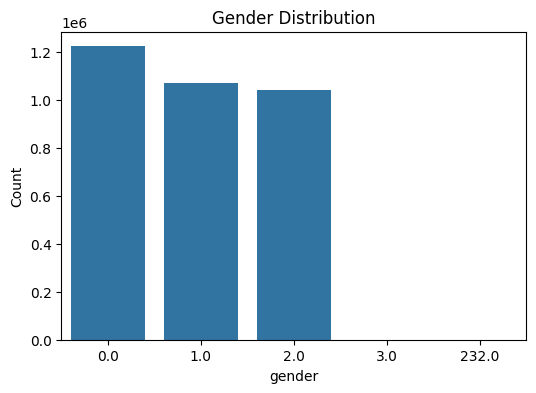
\includegraphics[width=0.68\linewidth]{figures/25.png}
    \caption{Trực quan hóa phân bố các giá trị của cột “gender”}
\end{figure}
\newpage
\textbf{c) Bảng teacher.json}\\
Sau đây là các thống số cơ bản của bảng
\begin{figure}[h]
    \centering
    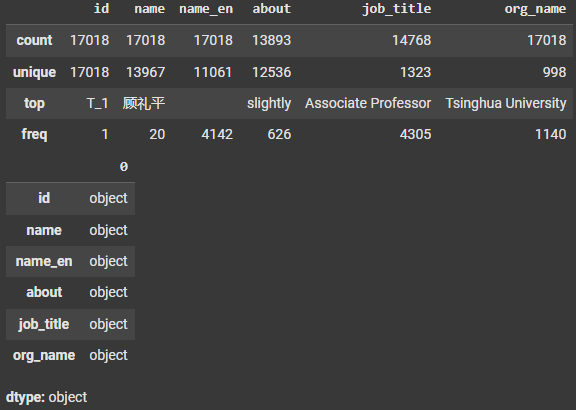
\includegraphics[width=0.6\linewidth]{figures/27.png}
\end{figure}\\
Tham khảo phân phối của top 10 tên việc xuất hiện nhiều nhất trong bảng
\begin{figure}[h]
    \centering
    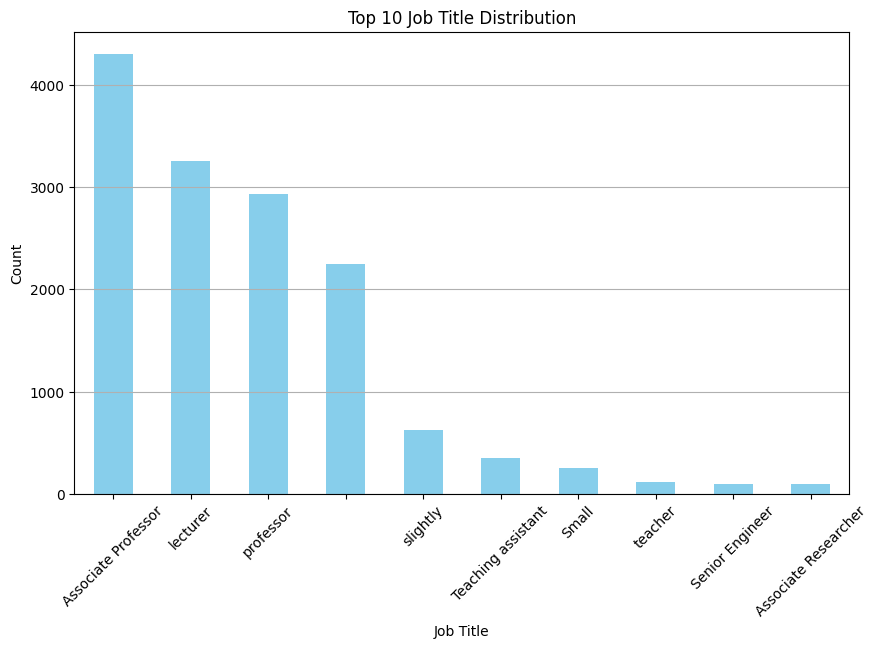
\includegraphics[width=0.75\linewidth]{figures/28.png}
\end{figure}\\
Tham khảo phân phối của top 10 tổ chức xuất hiện nhiều nhất trong bảng
\newpage
\begin{figure}
    \centering
    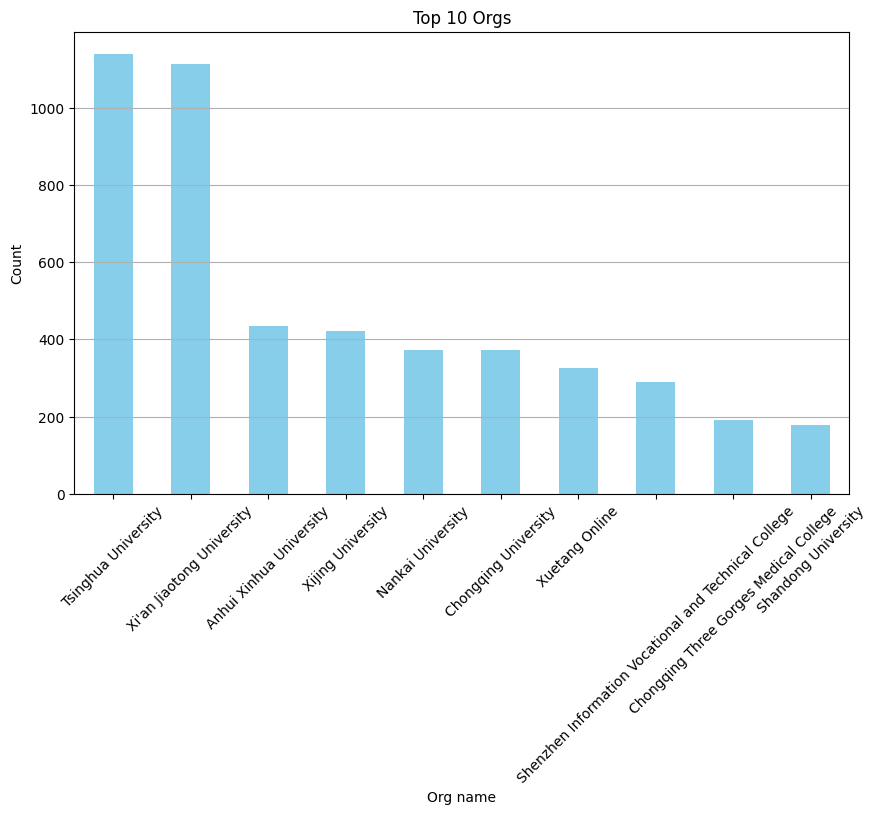
\includegraphics[width=0.75\linewidth]{figures/29.png}
\end{figure}
Ta thực hiện phân tích mối quan hệ giữa ba chức vụ (job titles) có số lượng giáo viên nhiều nhất và mười tổ chức (organizations) có số lượng giáo viên cao nhất
\begin{figure}[h]
    \centering
    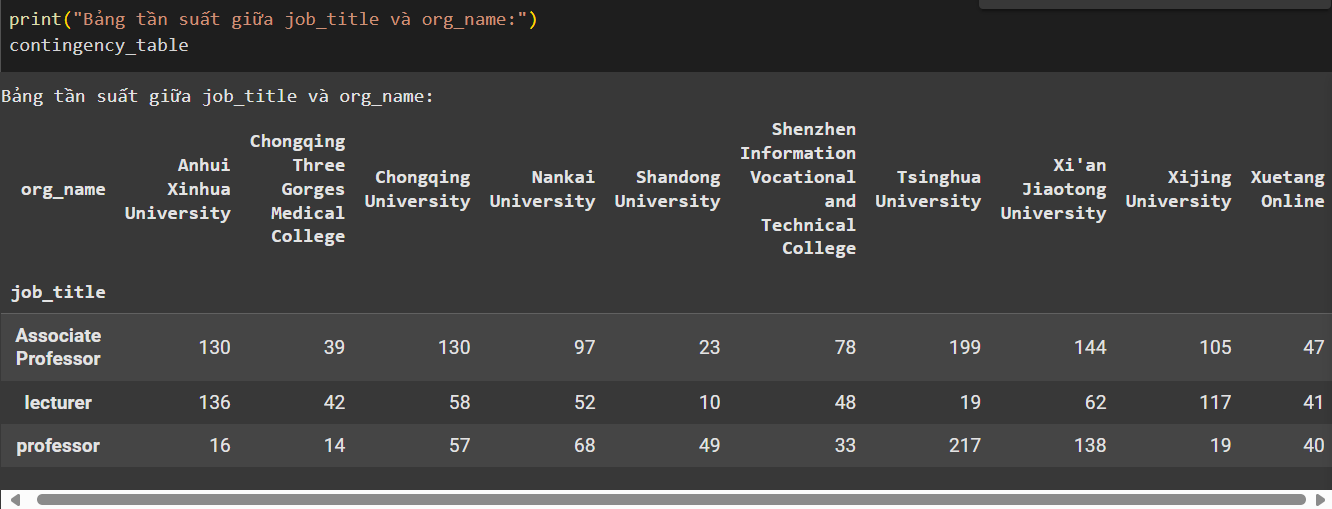
\includegraphics[width=0.95\linewidth]{figures/30.png}
\end{figure}
\newpage
\begin{figure}
    \centering
    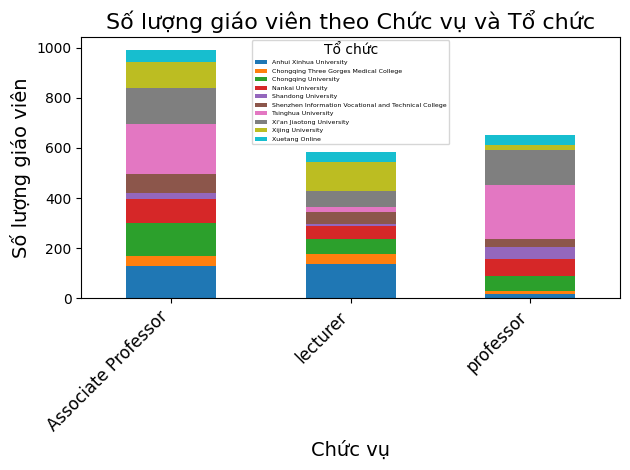
\includegraphics[width=0.65\linewidth]{figures/31.png}
\end{figure}
Sau khi lọc bỏ các liên kết có khóa học hoặc teacher không tồn tại dựa vào file course-teacher.txt, số hàng còn lại là 35593. Các thông tin được trực quan hóa như sau
\begin{figure}[h]
    \centering
    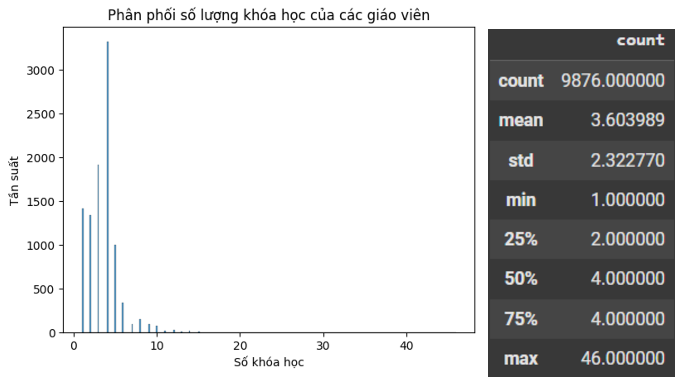
\includegraphics[width=0.8\linewidth]{figures/32.png}
    \caption{Histogram thể hiện số lượng khóa học của mỗi teacher và bảng thống kê mô tả tương ứng}
\end{figure}
\newpage
\begin{figure}
    \centering
    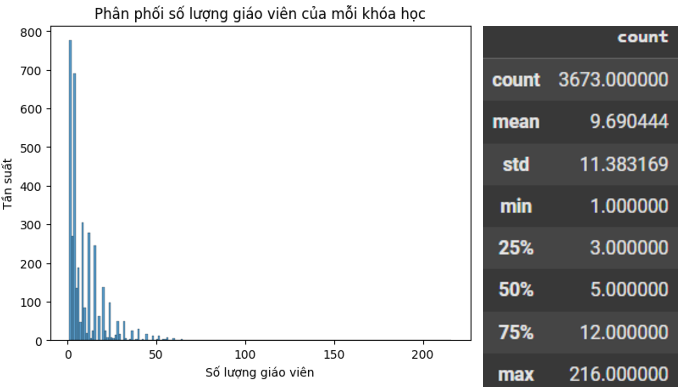
\includegraphics[width=0.8\linewidth]{figures/33.png}
    \caption{Histogram thể hiện số lượng teacher của mỗi khóa học và bảng thống kê mô tả tương ứng}
\end{figure}
\textbf{d) Bảng school.json}\\
Ta đếm dữ liệu ở từng cột, đếm các giá trị đặc biệt, giá trị xuất hiện nhiều nhất với tần số của nó:
\begin{figure}[h]
    \centering
    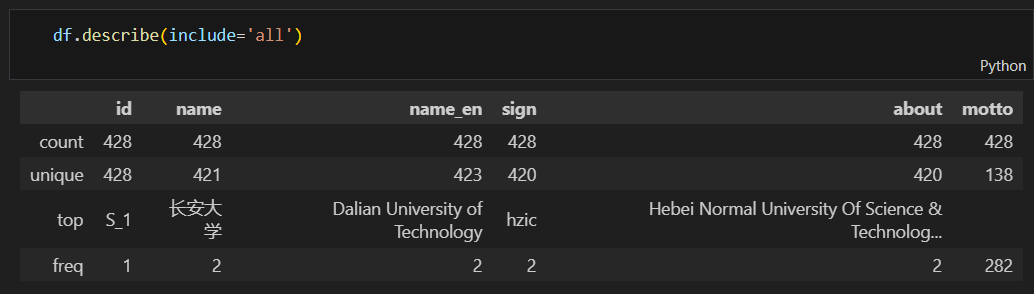
\includegraphics[width=0.75\linewidth]{figures/34.png}
\end{figure}\\
Kiểm tra kiểu dữ liệu của từng cột: 
\newpage
\begin{figure}
    \centering
    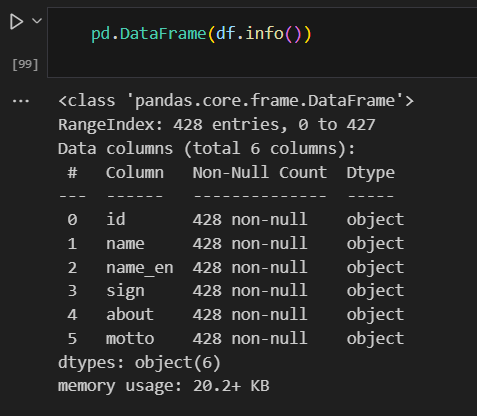
\includegraphics[width=0.6\linewidth]{figures/35.png}
\end{figure}
Ta tạo 2 cột mới là “about\_length” và “motto\_length” để lần lượt thể hiện độ dài của giá trị dữ liệu ở 2 cột “about” và “motto”:
\begin{figure}[h]
    \centering
    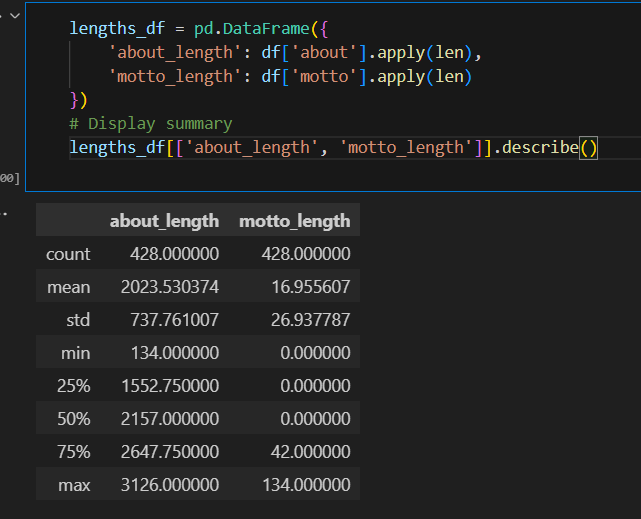
\includegraphics[width=0.65\linewidth]{figures/36.png}
\end{figure}
\newpage
Có 2 cột ta cần là “about\_length” và “motto\_length” để ta tìm phân bố độ dài của giá trị lên đồ thị:
\begin{figure}[h]
    \centering
    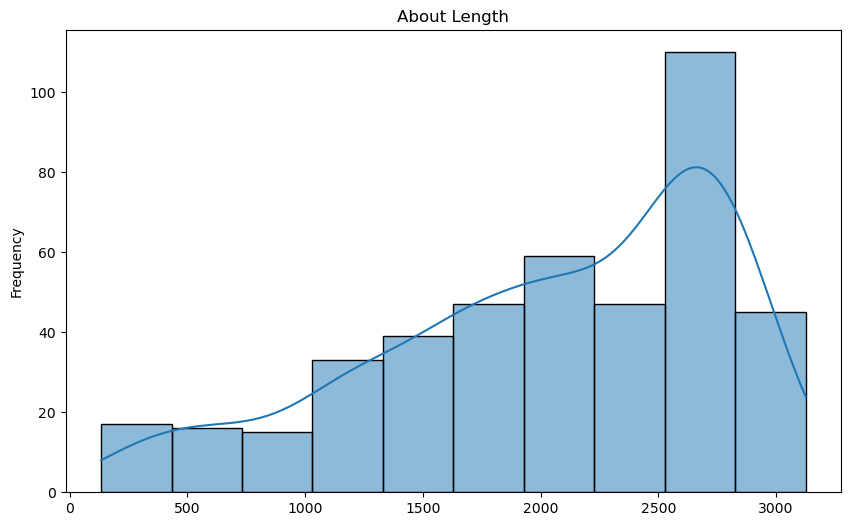
\includegraphics[width=0.7\linewidth]{figures/37.png}
\end{figure}\\
Dựa vào biểu đồ ta có thể nhận xét rằng mô tả của các trường đều rất chi tiết, số lượng trường với số lượng từ phần mô tả > 2000  chiếm phần lớn. Tuy nhiên thông tin này có vẻ không hữu ích với hệ thống khuyến nghị.
\begin{figure}[h]
    \centering
    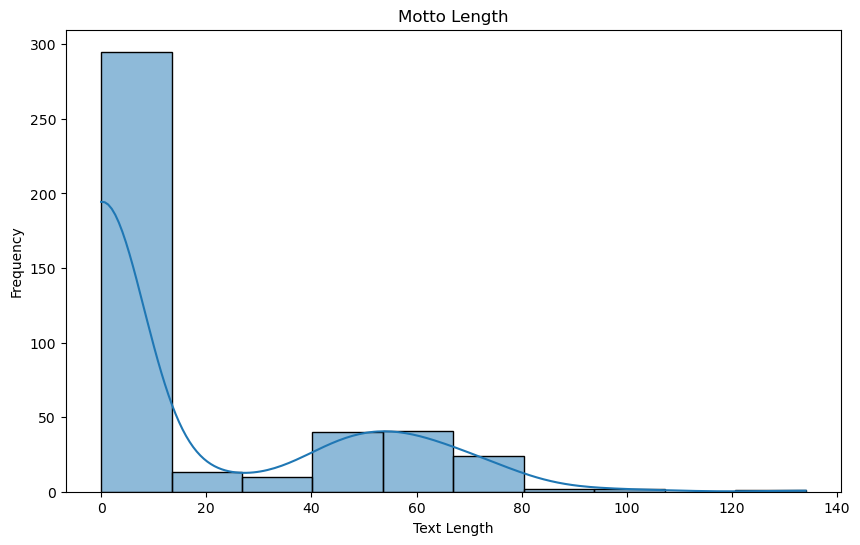
\includegraphics[width=0.7\linewidth]{figures/38.png}
\end{figure}\\
Hầu hết các trường đại học đều có một khẩu hiệu ngắn gọn dưới 20 từ vì chủ yếu khẩu hiệu sẽ đơn giản nhất có thể để truyền đạt tầm nhìn và mục tiêu của trường một cách trực tiếp ngắn gọn, đọng lại trong trí nhớ người xem. Một phần nhỏ hơn các trường có khẩu hiệu tương đối dài với 40 đến 88 chữ. 
\newpage
\textbf{e) Bảng course-field.json}
\begin{figure}[h]
    \centering
    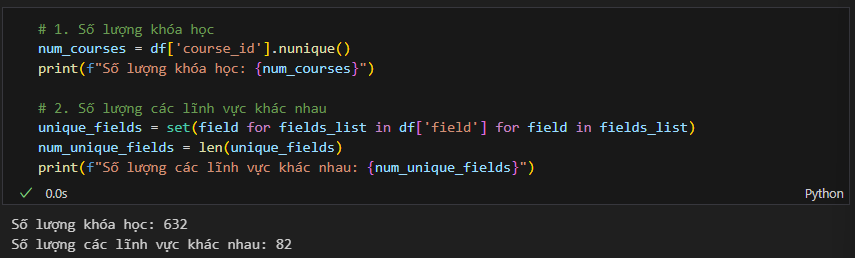
\includegraphics[width=1\linewidth]{figures/39.png}
    \caption{Tổng số lượng khóa học và tổng số lượng các lĩnh vực khác nhau}
\end{figure}
\begin{figure}[h]
    \centering
    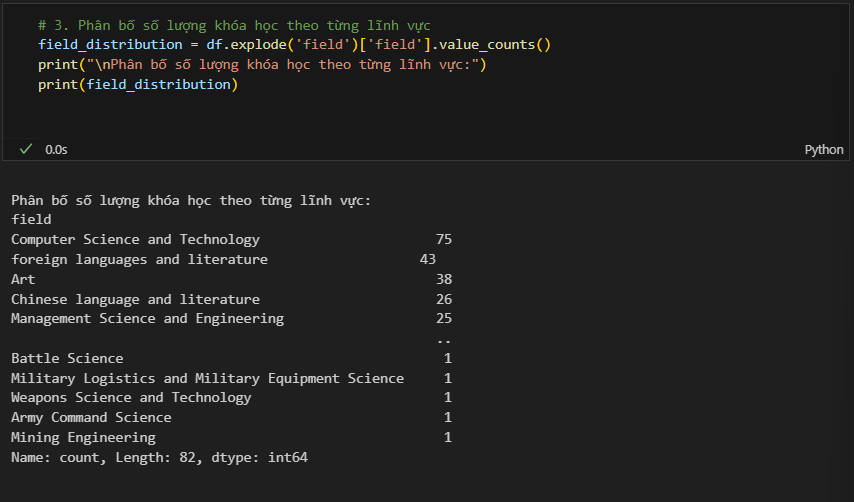
\includegraphics[width=1\linewidth]{figures/40.png}
    \caption{Phân bố số lượng khóa học theo từng lĩnh vực}
\end{figure}
\newpage
\begin{figure}
    \centering
    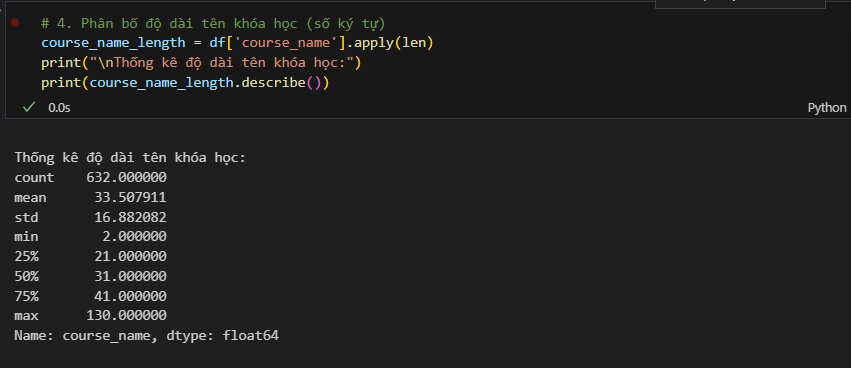
\includegraphics[width=0.85\linewidth]{figures/41.png}
    \caption{Phân bố độ dài tên khóa học}
\end{figure}
\begin{figure}[h]
    \centering
    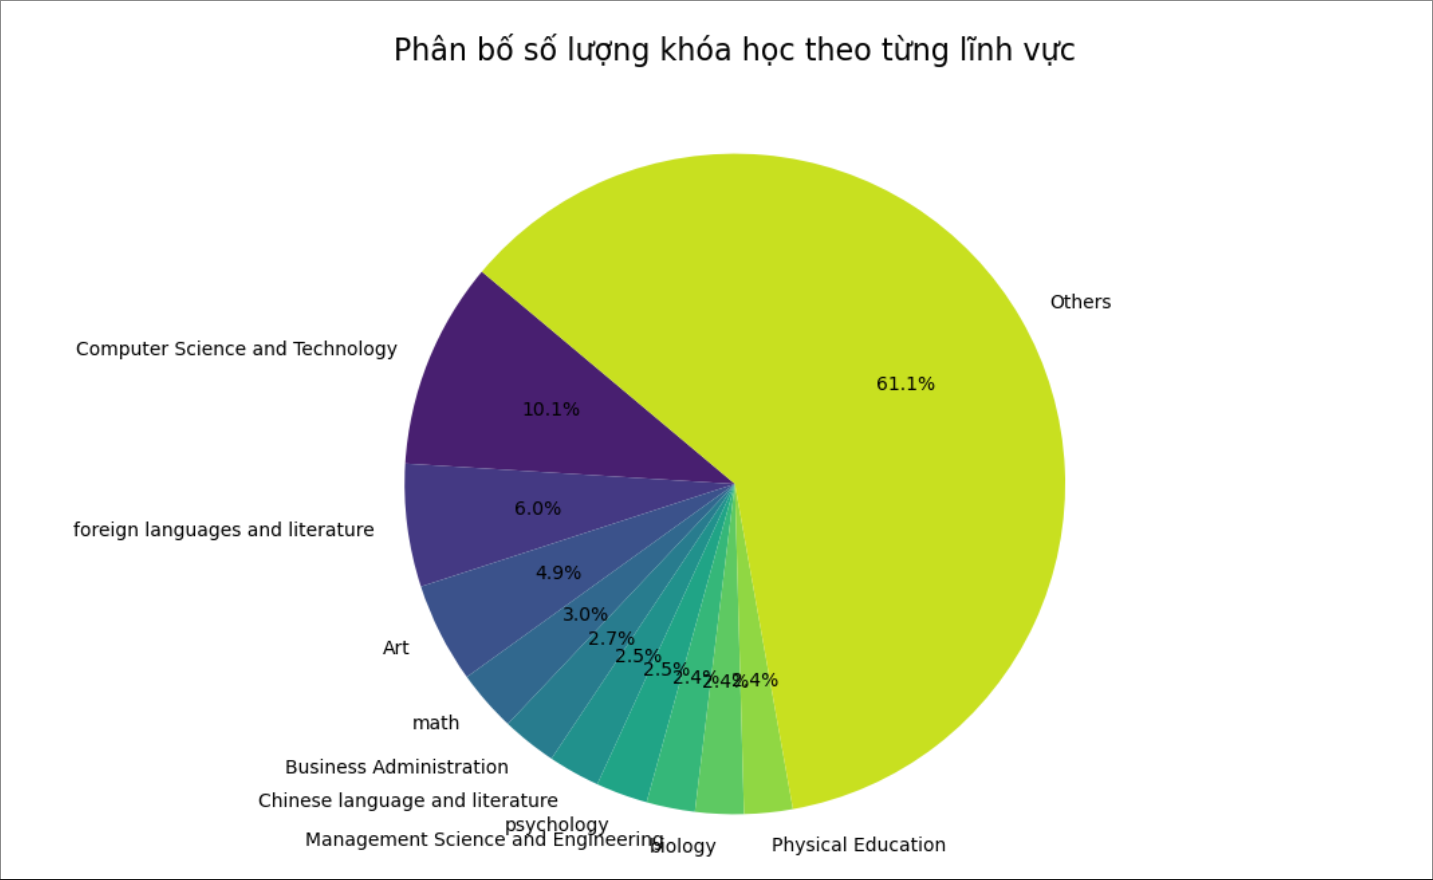
\includegraphics[width=0.9\linewidth]{figures/42.png}
    \caption{Biểu đồ thanh thể hiện sự phân bố số lượng khóa học theo từng lĩnh vực}
\end{figure}
\newpage
\begin{figure}
    \centering
    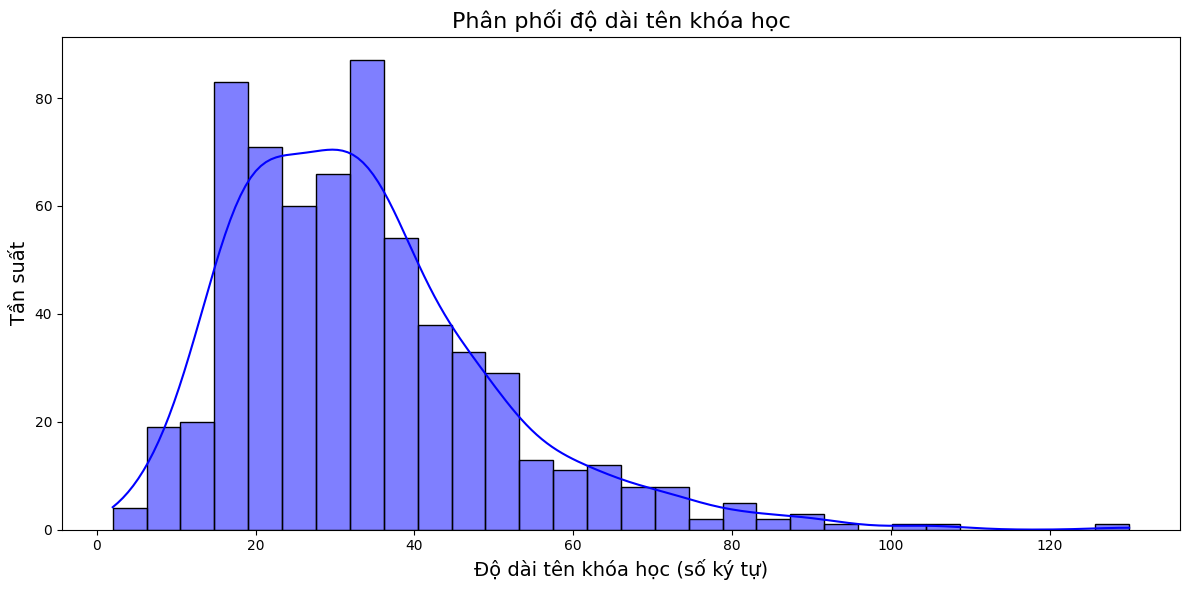
\includegraphics[width=0.75\linewidth]{figures/44.png}
    \caption{Biểu đồ phân phối cho độ dài tên khóa học}
\end{figure}
\subsubsection{Làm sạch dữ liệu}
\textbf{a) Bảng course.json}\\
Ta kiểm tra dữ liệu thiếu, dữ liệu không nhất quán, dữ liệu trùng lặp và dữ liệu trống:
\\
Đầu tiên ta thấy được có 647 giá trị ở cột “name\_trans” bị trùng lặp cho dù id không bị trùng, chứng tỏ có sự lỗi nhất định trong bộ dữ liệu, cũng như nãy đã thống kê ta thấy được có rất nhiều giá trị trống ở cột “field\_trans”.\\
\\
Ta kiểm tra kĩ hơn về các dòng có giá trị trong cột “name” bị trùng lặp:
\begin{figure}[h]
    \centering
    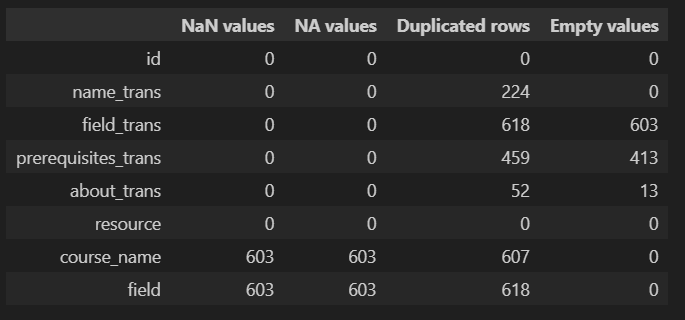
\includegraphics[width=1\linewidth]{figures/26.png}
\end{figure}
\newpage
\begin{figure}
    \centering
    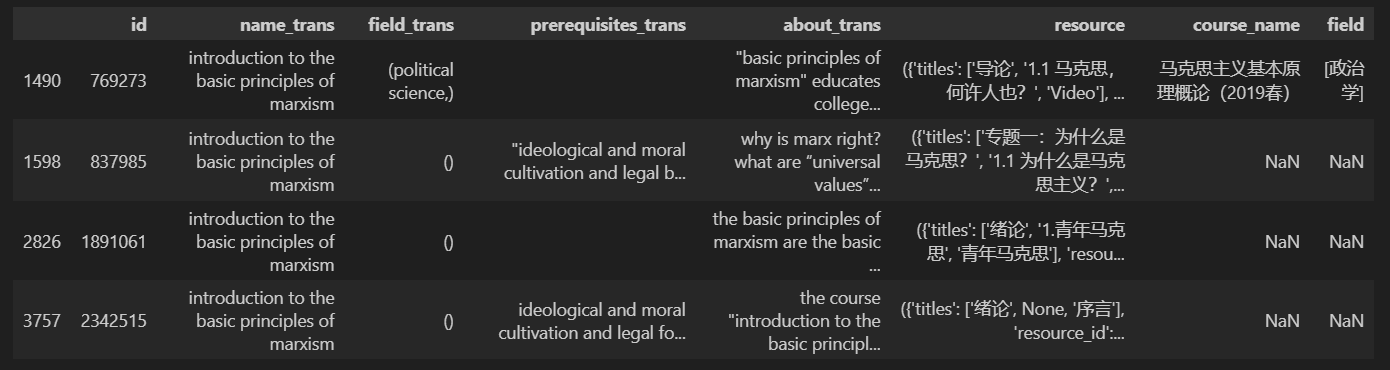
\includegraphics[width=1\linewidth]{figures/45.png}
\end{figure}
Ta thấy được đa số dữ liệu trong này cột “field” đa số bị trống và trùng lặp, cũng như các cột khác không có ý nghĩa hoặc trùng với các cột khác, thực hiện chi square test, ta có được kết quả với P-value rất thấp, chứng tỏ các giá trị phụ thuộc với nhau chứ không hề có giá trị mới. Chứng tỏ ta có thể xoá được các dòng dữ liệu này, cũng như các khoá học không tồn tại trong “course-field.json”.\\
\textbf{b) Bảng user.json}\\
Ta thấy cột “year\_of\_birth” bị thiếu dữ liệu hơn 97\% trong khi các cột còn lại tỉ lệ \% thiếu là rất thấp. Ta tiến hành loại bỏ cột này, sau đó ta sẽ tiến hành xử lý dữ liệu nhiễu trên cột gender với 2 giá trị nhiễu là 232 và 3\\
\textbf{c) Bảng concept.json}\\
Ta thấy cột “id” bị thiếu 207 giá trị, ta tiến hành bỏ các hàng này.\\
\begin{figure}[h]
    \centering
    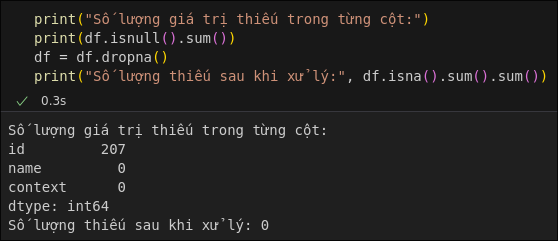
\includegraphics[width=1\linewidth]{figures/46.png}
\end{figure}
\newpage
Ta kiểm tra kĩ hơn về các bản ghi có giá trị trùng lặp và xử lý chúng:\\
\begin{figure}[h]
    \centering
    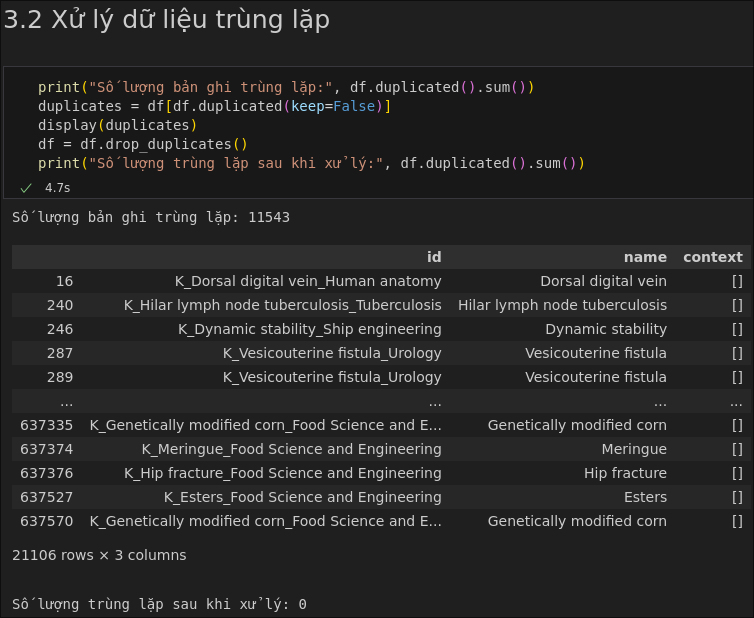
\includegraphics[width=1\linewidth]{figures/47.png}
\end{figure}\\
\textbf{d) Bảng course-field.json}\\
Sử dụng isnull().sum() để tính số lượng giá trị thiếu trong từng cột. Sau đó loại bỏ hàng chứa giá trị thiếu bằng cách sử dụng dropna()
\newpage
\begin{figure}
    \centering
    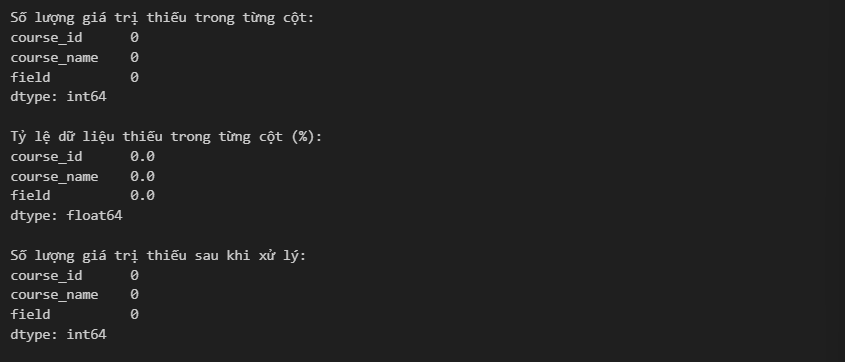
\includegraphics[width=1\linewidth]{figures/48.png}
\end{figure}
Dữ liệu văn bản thường chứa nhiều thông tin nhiễu chẳng hạn như các ký tự không mong muốn: Các ký tự đặc biệt, dấu câu, hoặc ký tự không phải chữ cái có thể làm giảm chất lượng phân tích. Ở đây chúng ta sẽ tiến hành loại bỏ các ký tự không cần thiết, các khoảng trắng dư thừa và thường hóa các ký tự viết hoa\\
\\
Để kiếm tra dữ liệu trùng lặp, chúng ta sử dụng phương thức duplicated() trong pandas. Đầu tiên xác định các bản ghi trùng lặp, sau đó đếm số lượng và hiển thị các bảng ghi trùng lặp đó. Sau đó tiến hành xóa bản ghi trùng lặp bằng cách sử dụng drop\_duplicates()
\newpage
\begin{figure}
    \centering
    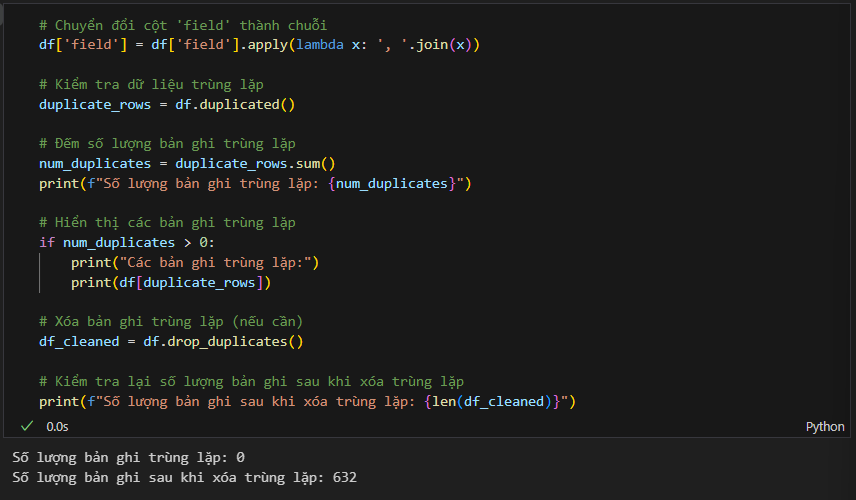
\includegraphics[width=1\linewidth]{figures/49.png}
\end{figure}
\textbf{e) Bảng school.json}\\
Ta xoá cột “name” đi vì trùng với ý nghĩa với cột “name\_en” (tên nhưng trong Tiếng Anh)\\
\\
Ta thống nhất cột “sign” (kí hiệu đại diện cho trường) đều là tất cả in hoa:
\newpage
\begin{figure}
    \centering
    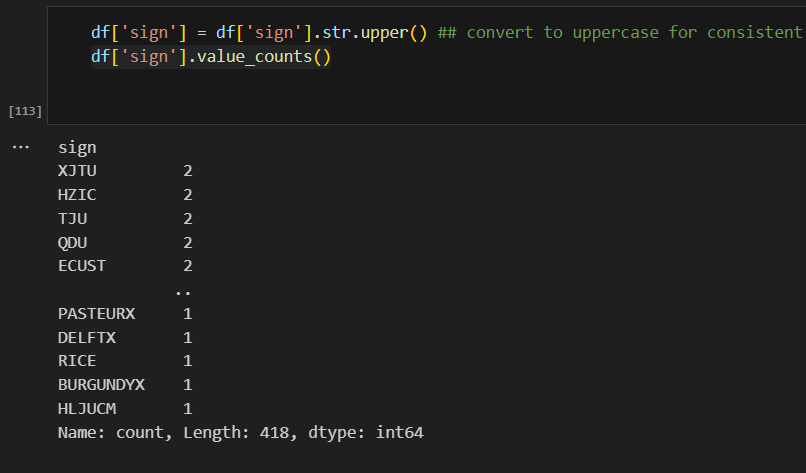
\includegraphics[width=0.7\linewidth]{figures/50.png}
\end{figure}
Vì ở đây tên trường (“name\_en”) cũng như kí hiệu (“sign”) là chìa khoá chính, hay nói cách khác là giá trị duy nhất nên không thể có dòng trùng với nhau, ta tiến hành xoá các dòng trùng giá trị:
\begin{figure}[h]
    \centering
    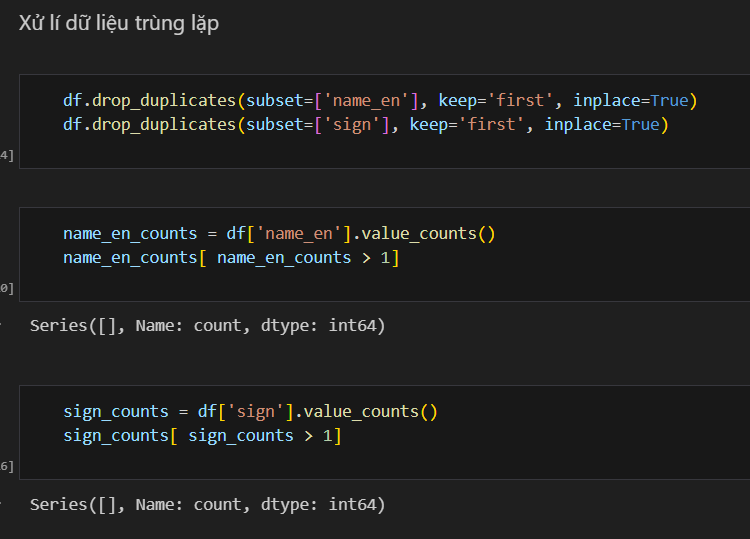
\includegraphics[width=0.7\linewidth]{figures/51.png}
\end{figure}\\
\textbf{g) Bảng teacher.json}\\
Ở đây có cột name\_en bị thiếu nên điền vào cột đó bằng cách lấy phiên âm của cột name là được. Để làm việc này có thể sử dụng thư viện pypinyin để lấy phát âm dùng cho tên tiếng anh.
\newpage
\begin{figure}
    \centering
    \includegraphics[width=0.8\linewidth]{figures/52.png}
\end{figure}
\subsubsection{Chuyển đổi dữ liệu}
\textbf{Feature Engineering:}
Nhóm sẽ chọn các bảng và thuộc tính có thể sử dụng để tạo ra feature các mô hình khuyến nghị dựa trên bộ dữ liệu đã xử lý và làm sạch trước đó:\\
\\
Các bảng được chọn và thuộc tính sử dụng:
\begin{figure}[h]
    \centering
    \includegraphics[width=0.6\linewidth]{figures/53.png}
\end{figure}
\newpage
\begin{itemize}
    \item Với ‘user.json’: ‘course\_order’ gồm các khóa học mà user đã đăng ký với khóa học sau cùng là khóa học gần đây nhất, dùng để tạo liên kết giữa ‘user.json’ và ‘course.json’.
    \item Với ‘course.json’: Đây là table quan trọng chứa thông tin về các khóa học như ‘name’, ‘about’ và ‘field’.
    \item Với ‘teacher.json’, ‘school.json’: dùng để tạo relation với ‘course.json’ chứa thông tin về trường tổ chức khóa học và giáo viên giảng dạy.
    \item Với ‘course-field.json’: chứa các field của mỗi khóa học, dùng để kiểm tra với trường ‘field’ trong ‘course.json’.
    \item Với ‘concept.json’: id theo quy ước ‘K\_{concept name}{field}’, tạo thêm feature concept-name\_field với mỗi khoá học.
\end{itemize}
Tạo knowledge graph:
\begin{figure}[h]
    \centering
    \includegraphics[width=0.3\linewidth]{figures/54.png}
\end{figure}\\
Tạo interaction giữa người dùng với khóa học: sử dụng 5-core filtering, lọc người dùng với ít hơn 5 khóa học và những khóa học có số lượng đăng ký dưới 5.\\
\\
Kết quả: Vì data đã được xử lý trước đó nên ta thấy không có thay đổi đáng kể
\begin{center}
\begin{tabular}{|| m{15em}  m{15em}||} 
 \hline
 Trước khi filter & Sau khi filter\\ [0.5ex] 
 \hline\hline
 1.183.774 interactions & 1.182.745 interactions \\ [1ex]
 \hline
\end{tabular}
\end{center}
\newpage
Tạo relation giữa các entities: course-relation-attribute. Sau đó ta tiến hành lọc theo tiêu chí, số lần course xuất hiện tối thiểu là 5 và số lần xuất hiện tối thiểu của một relation là 25. \\
\\
Kết quả: 
\begin{center}
\begin{tabular}{|| m{15em}  m{15em}||} 
 \hline
 Trước khi filter & Sau khi filter\\ [0.5ex] 
 \hline\hline
 376.093 interactions & 71.787 interactions \\ [1ex]
 \hline
\end{tabular}
\end{center}
\subsubsection{Chia tập dữ liệu}
\begin{itemize}
    \item Dữ liệu cuối cùng được chia theo chiến lược leave-one-out: Với mỗi user, nhóm giữ khoá học cuối cùng làm test, các khoá học còn lại làm train. 
    \item Dữ liệu cuối cùng để thực nghiệm có 4 loại dữ liệu chính: dữ liệu thô (chưa xử lí), 10\% dữ liệu thô, dữ liệu đã xử lí (chiến lược leave-one-out) và 10\% dữ liệu đã xử lí.
\end{itemize}

\subsection{Độ đo đánh giá}
\subsection{Kịch bản thực nghiệm}
\subsection{Đánh giá kết quả thực nghiệm}
